\section{Motivation} \label{sec:motivation}
Clock frequency determines the accelerator operation speed 
and directly affects the performance. Accordingly, it also has influence on the 
neural network runtime and energy efficiency. In this section, we take 
an open-sourced CNN accelerator named PipeCNN \cite{pipecnn_2} as an example and analyze the 
influence of clock frequency on the neural network performance and energy efficiency.

The accelerator is implemented on KCU1500 and attached to a desktop computer with 
Intel i7-6700@3.40GHz. The basic convolution structure is shown in Fig \ref{fig:cnn-arch}. 
The computing array consists of 16 dot production units which is also named as 
processing elements (PE). Each PE allows a parallel dot production of two 4-data vectors.
The optimized clock frequency according to the SDAccel compilation 
is 200 MHz. 

\begin{figure}
	\center{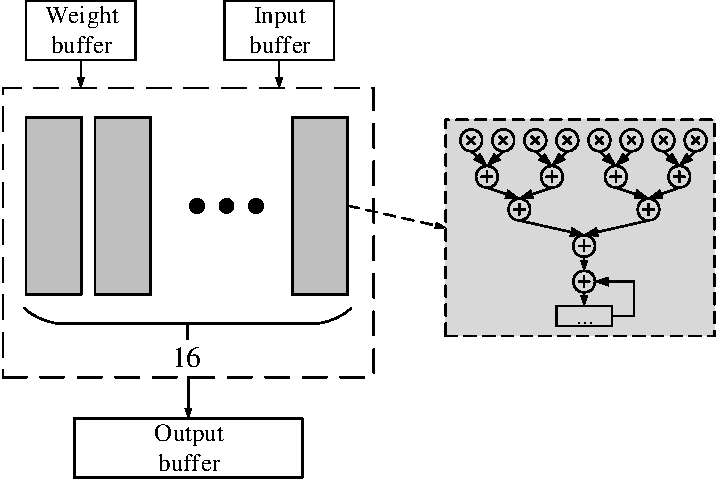
\includegraphics[width=0.65\linewidth]{accelerator}}
    \caption{Baseline CNN accelerator architecture.}
\label{fig:cnn-arch}
\vspace{-1em}
\end{figure}

In order to evaluate the influence of clock 
frequency, we set the clock to 50 MHz, 100 MHz, and 150 MHz respectively.
A set of neural networks including LeNet, AlexNet, VGG-16 and VGG-19 are used as the benchmark.
Both the runtime and energy efficiency are normalized to the 50 MHz implementation.
Normalized runtime of the neural network benchmark executed on the accelerators are 
shown in Fig \ref{fig:computing-bound}. It shows that the 
overall performance of the neural network benchmark
almost increases proportional to the clock frequency. 
It can be predicted that the processing remains 
computing-bound and high-frequency CNN accelerator 
design will be beneficial.

\begin{figure}
	\center{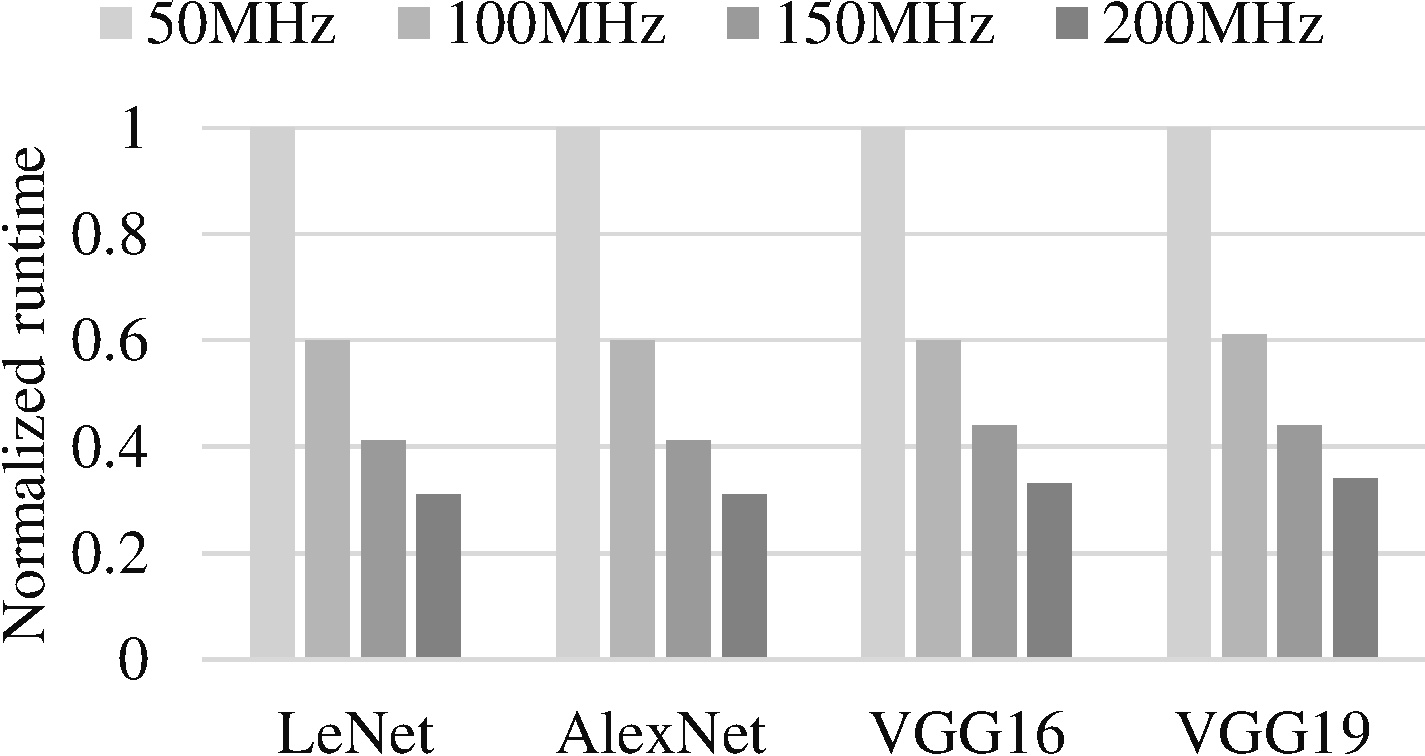
\includegraphics[width=0.65\linewidth]{relative_time}}
    \caption{Normalized runtime of neural networks executed on CNN accelerators with different clock frequency.}
\label{fig:computing-bound}
\vspace{-1em}
\end{figure}

To analyze the energy consumption, we obtain the power consumption from SDAccel 2017.1. 
Given the power consumption and the runtime, 
we calculated the energy delay product (EDP) which can be used as an energy efficiency metric.
The experiment result is presented in Fig \ref{fig:edp}.
It shows that higher clock frequency 
enhances both the neural network performance and energy efficiency. 
This motivates the use of overclocking that enables even higher clock frequency.


\begin{figure}
	\vspace{-1em}
	\center{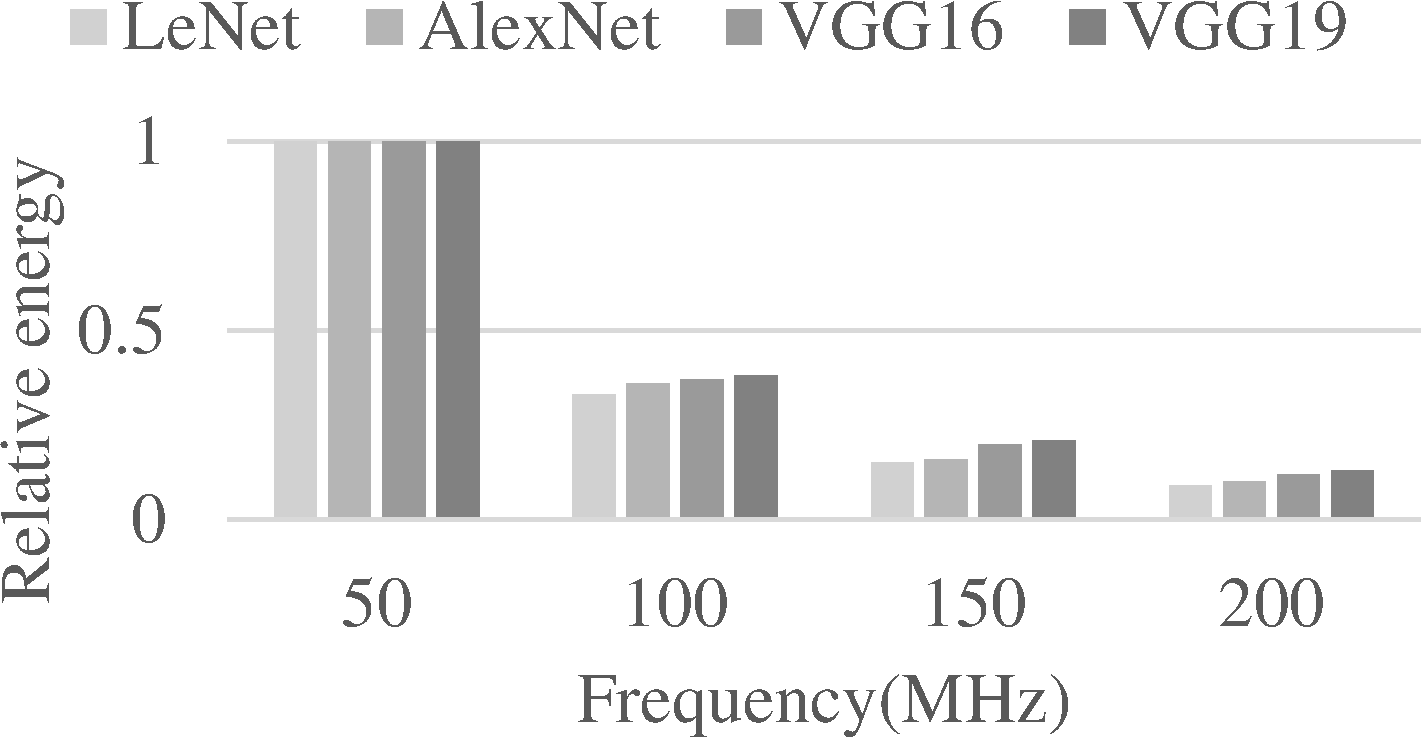
\includegraphics[width=0.65\linewidth]{relative_energy}}
    \caption{Normalized EDP of neural networks executed on CNN accelerators with different clock frequency.}
\label{fig:edp}
\vspace{-1em}
\end{figure}


